% Chapter 04 - Reaction Mechanisms.tex
% Copyright (c) 2014 - 2016, zhiayang@gmail.com
% Licensed under the Apache License Version 2.0.


\pagebreak
\part{Reaction Mechanisms}

	The reaction mechanism of any given reaction allows one to glean more information than usually possible from just the chemical equation.
	The chemical equation simply represents the overall reactants and products of the reaction; the reaction mechanism on the other hand
	represents the individual steps of the reaction, including which molecules collide with with other molecules, and the intermediate
	compounds that are formed.

	The mechanism of any given reaction cannot be directly determined; they must first be hypothesised, and then confirmed with data from
	experiments.


	\section{Single-step Reactions}

		For single-step reactions, there is only one step, so naturally it has to be the \textit{rate-determining}, or \textit{slow}, step.
		There are no intermediates either.

		Since the one equation represents the entire reaction, then the stoichiometric coefficients of each reactant \textit{are} their
		orders. For example,

		\txtdiagram{
			\schemestart[0, 1.0, thick]
				2 A + B
				\arrow
				C
			\schemestop
		}{Rate = k[A]\sps{2}[B]\sps{1}}

		Again, note that this is only applicable to the \textit{rate-determining} step, the orders of reaction for each reactant cannot be
		determined from the overall equation.

	% end section



	\pagebreak
	\section{Multi-step Reactions}

		Even though most reactions appear to be single-step, they often consist of multiple steps in reality. The rate of reaction of the entire
		system is governed, naturally, by the \textit{rate-determining step}; this step is often slow because of a high activation energy.

		For multi-step reactions, the order of reaction of each reactant is determined by their stoichiometric ratio in the
		\textit{rate-determining step}, not in the overall reaction.

		\subsection{Elementary Steps}

			In a multi-step reaction, the mechanism is often split into multiple \textit{elementary reactions} --- those that cannot be broken down
			further into separate steps.

			\begin{bulletlist}
				& Unimolecular steps involve only one molecule.
				& Bimolecular steps involve the collision of two molecules.
				& Termolecular steps involve the collision of three molecules, simultaneously.
			\end{bulletlist}

			Given that termolecular reactions are already quite rare, there are no known elementary steps involving the collision of four or
			more molecules, simultaneously.

		% end subsection


		\subsection{Intermediates}

			Intermediates, distinct from transition states, are typically stable compounds that can often be isolated, and are usually formed
			as the product of intermediate steps in the reaction mechanism.

			Intermediates must be reacted away by the end of the reaction, since they are not present in the overall equation.

		% end subsection


		\pagebreak
		\subsection{Mechanisms}

			For multi-step reactions, it is important to note that reactants in the elementary (fast) steps \textit{before} the
			rate-determining step are included in the rate equation, and reactants appearing in the fast steps \textit{after} the
			rate-determining step are \textit{not} included.

			Thus, there are two main cases --- the rate-determining step is the first step, and when it is not.

			\subsubsection{Rate-Determining Step is First}

				For example, take the reaction between nitrogen dioxide (\ch{NO2}) and fluorine gas (\ch{F2}):

				\txtdiagram{
					\schemestart[0, 1.5, thick]
						\ch{NO2} + \ch{F2}\arrow{->[\tinytext{Step 1 (slow)}]}\ch{NO2F} + \ch{F}
						\arrow(@c1.south east--.north east){0}[-90,.35]
						\ch{NO2} + \ch{F}\arrow{->[\tinytext{Step 2 (fast)}]}\ch{NO2F}
						\arrow(@c3.south east--.north east){0}[-90,.35]
						\ch{2 NO2} + \ch{F2}\arrow{->[\tinytext{Overall}]}\ch{2NO2F}
					\schemestop
				}{Rate = k[\ch{NO2}][\ch{F2}]}

				As can be seen, the orders of reaction of \ch{NO2} and \ch{F2} follow the coefficients in the rate-determining slow
				step, not the overall equation. This is the case for a reaction where the slow step is the first step.

			% end subsubsection


			\subsubsection{Rate-Determining Step is not First}

				If the rate-determining step is not the first step, then the reaction most likely involves an intermediate, which must be
				dealt with before the final step, since it cannot appear in the overall reaction.

				For example, taking the reaction for the oxidation of nitrogen monoxide (\ch{NO}),

				\txtdiagram{
					\schemestart[0, 1.5, thick]
						\ch{NO} + \ch{O2}\arrow{<=>[\tinytext{Step 1 (fast, reversible)}]}\ch{NO3}
						\arrow(@c1.south east--.north east){0}[-90,.35]
						\ch{NO3} + \ch{NO}\arrow{->[\tinytext{Step 2 (slow)}]}\ch{2 NO2}
						\arrow(@c3.south east--.north east){0}[-90,.35]
						\ch{2 NO} + \ch{O2}\arrow{->[\tinytext{Overall}]}\ch{2 NO2}
					\schemestop
				}{\vspace{-2em}}

				In this situation, the intermediate species \ch{NO3} is formed in the first fast step, but is reacted away in the second,
				slow step. To begin with, a preliminary rate equation comprising the reactants in the slow step can be formed:

				\txtdiagram{
					Rate = k\sbs{1}[\ch{NO3}][\ch{NO}]
				}{\vspace{-2em}}

				The concentration of NO3 must be substituted for the concentrations of the reactants that it was created from, in this case
				\ch{NO} and \ch{O2}. Since the first step is an equilibrium reaction, the equilibrium constant \Kc can be used to calculate
				[\ch{NO3}] in terms of [\ch{NO2}] and [\ch{O2}].

				\diagram[1.5]{
					$K_{c} = \frac{[NO_{3}]}{[NO][O_{2}]}$
				}

				Moving things around, we get this:

				\diagram[1.5]{
					$[NO_{3}] = K_{c}[NO][O_{2}]$
				}

				Thus, substituting this into the original, partial rate equation and refactoring $k = k_{1} \times K_{c}$:

				\diagram[1.5]{
					\schemestart[0, 1.5, thick]
						$Rate$ \arrow{0}[,.05] $= k_{1}K_{c}[NO][O_{2}][NO]$
						\arrow(@c1.south east--.north east){0}[-90,.2]
						\arrow{0}[,.05] $= k[NO]^{2}[O_{2}]$
					\schemestop
				}

				By looking at the reaction, it might be tempting to come to the conclusion that, because \SI{1}{\mole} of \ch{NO3} is formed by
				\SI{1}{\mole} of \ch{NO} and \ch{O2}, it is possible to simply substitute $[NO_{3}] = [NO][O_{2}]$ directly. This is, however,
				incorrect.

				Don't do it.

			% end subsubsection


			\pagebreak
			\subsubsection{Reaction Pathway Diagram}

				\diagram[1.0]{
					\begin{endiagram}[scale=2.0,offset=1.5,x-label-text=reaction pathway,y-label-text=energy]
						\ENcurve[step=1.5]{2, 4.5, 3, 5.5, 0}

						\ShowNiveaus[shift=-1.0,length=2.0,niveau=N1-1]
						\ShowNiveaus[shift=0.0,length=2.0,niveau=N1-3]
						\ShowNiveaus[shift=1.0,length=2.0,niveau=N1-5]

						\ShowEa[label, label-side=left, label-pos=0.6, from={(N1-1) to (N1-2)}]
						\ShowEa[label, label-side=left, label-pos=0.6, from={(N1-3) to (N1-4)}]
						\ShowGain[label,offset=-40mm]

						\draw[above] (N1-1) ++ (1,0) node {\small \hspace{-40mm}reactants};
						\draw[below] (N1-3) ++ (0,0) node {\small intermediates};
						\draw[above] (N1-5) ++ (1,0) node {\small products};

					\end{endiagram}
				}

				The diagram is mostly self-explanatory; there is an \textit{intermediate compound} formed between the formation of the products.
				The intermediate is \textit{not the same} as a transition state --- the former is at a local energy minimum, while the latter
				is at a local energy maximum. Intermediates can sometimes be isolated as compounds, while transitions states can never be.

			% end subsubsection

		% end subsection

	% end section










	\pagebreak
	\section{Catalysis of Reactions}

		As explained previously, catalysts provide an alternative reaction pathway for the reaction, typically with a lower activation energy.
		There are two mechanisms of action for catalysis: homogeneous catalysts and heterogeneous catalysts.

		The mechanism of action of the catalyst is determined by the phase it is in. Note that \textit{phase} and \textit{state} are
		different concepts. While each state represents a phase, an oil phase and an aqueous phase are different phases, but the same state.

		Note that the concentration of a catalyst over the course of the reaction does not decrease, since it must be regenerated at the end of
		the reaction.


		\subsection{Homogeneous Catalysts}

			Homogeneous catalysts exist in the same phase as the reactants of the reaction. They are uniformly mixed in the reaction mixture,
			and they often form intermediates together with the reactants, before they are regenerated in the last step of the reaction.

			\diagram[1.0]{
				\begin{endiagram}[scale=2.0,offset=1.5,x-label-text=reaction pathway,y-label-text=energy]
					\ENcurve[step=4]{2, 5.0, 0}
					\ENcurve[tikz={red}]{2, 4.5[1], 3, 3.5[-1], 0}

					\ShowEa[label, label-side=left, label-pos=0.6, from={(N1-1) to (N1-2)}]
					\ShowEa[label, label-side=left, label-pos=0.6, from={(N2-1) to (N2-2)}]

					\ShowNiveaus[shift=-1.0,length=2.0,niveau=N1-1]
					\ShowNiveaus[shift=1.0,length=2.0,niveau=N1-3]

					\ShowGain[label,offset=-30mm]

					\draw[above] (N1-1) ++ (1,0) node {\small \hspace{-40mm}reactants};
					\draw[above] (N1-3) ++ (1,0) node {\small products};

				\end{endiagram}
			}

			In the diagram above, the catalysed reaction is represented with the red line. It can have any number of intermediates, as long
			as the  maximum activation energy is less than the activation energy of the original reaction.

			Homogeneous catalysts must be one of the reactants in the rate-determining step for it to affect the rate of reaction. As such,
			it usually appears in the final rate equation (for the catalysed reaction), even though it is not part of the balanced
			chemical equation.


			\subsubsection{Catalysis of \ch{I-} + \ch{S2O8^2-} reaction with \ch{Fe^2+}}

				\ch{Fe^2+} acts as a catalyst in the reaction of iodide ions (\ch{I-}) with peroxodisulphate ions (\ch{S2O8^2-}), via homogeneous
				catalysis. The reaction of these two species involves the collision of two negatively charged ions, which has a high energy barrier and
				thus is infeasible. As such, the reaction occurs very slowly without a catalyst.

				In this reaction, \ch{I-} is a reducing agent, and \ch{S2O8^2-} is an oxidising agent. However, with \ch{Fe^2+} as the catalyst,
				these two species do not interact directly. Instead, the positively charged \ch{Fe^2+} and \ch{Fe^3+} ions easily attract the
				negative ions, and it is oxidised and reduced by \ch{S2O8^2-} and \ch{I-} respectively.

				\txtdiagram{
					\schemestart[0, 1.5, thick]
						\ch{2 Fe^2+} + \ch{S2O8^2-}\arrow{->[\tinytext{Step 1}]}\ch{2 Fe^3+} + \ch{2 SO4^2-}
						\arrow(@c1.south east--.north east){0}[-90,.35]
						\ch{2 Fe^3+} + \ch{2 I-}\arrow{->[\tinytext{Step 2}]}\ch{I2} + \ch{Fe^2+}
						\arrow(@c3.south east--.north east){0}[-90,.35]
						\ch{S2O8^2-} + \ch{2 I-}\arrow{->[\tinytext{Overall}]}\ch{I2} + \ch{2 SO4^2-}
					\schemestop
				}{\vspace{-2em}}

				In the first step, \ch{Fe^2+} is oxidised by \ch{S2O8^2-} to form \ch{Fe^3+}. In the second step, this \ch{Fe^3+} is reduced
				again by \ch{I-} back to \ch{Fe^2+}, regenerating the catalyst. Since this involves the reaction of oppositely charged ions,
				the activation energy for each step is much lower than that for the uncatalysed reaction.

			% end subsubsection


			\subsubsection{Catalysis of oxidation of \ch{SO2} with \ch{NO2}}

				In the atmosphere, nitrogen dioxide often catalyses the oxidation of \ch{SO2} to \ch{SO3}, thus
				forming acid rain (mainly \ch{H2SO4}). It is catalysed in two steps:

				\txtdiagram{
					\schemestart[0, 1.5, thick]
						\ch{SO2} + \ch{NO2}\arrow{->[\tinytext{Step 1}]}\ch{SO3} + \ch{NO}
						\arrow(@c1.south east--.north east){0}[-90,.35]
						\ch{NO} + \ch{\fracHalf O2}\arrow{->[\tinytext{Step 2}]}\ch{NO2}
						\arrow(@c3.south east--.north east){0}[-90,.35]
						\ch{SO2} + \ch{\fracHalf O2}\arrow{->[\tinytext{Overall}]}\ch{SO3}
					\schemestop
				}{}

				The \ch{SO3} formed reacts readily with water vapour in the atmosphere to form sulphuric acid, \ch{H2SO4}.

			% end subsubsection

		% end subsection



		\subsection{Heterogeneous Catalysis}

			Heterogeneous catalysts catalyse the reaction from a different state or phase than the reactants in the reaction. It is most
			often a solid catalyst reacting with liquid or gaseous reactants. Thus, since they do not have a concentration, they do not
			appear in the rate equation; their effect is manifested in the rate constant $k$.

			Most heterogeneous catalysts have the concept of \textit{active sites}, which are areas on the surface of the solid catalyst
			that are available for reaction. Thus, catalysts with a larger surface area, such as wire gauze or fine powder, are preferred to
			increase the rate of reaction.

			\begin{bulletlist}
				& Haber Process for production of \ch{NH3} (ammonia) (\ch{Fe} powder or \ch{Fe2O3})
				& Hydrogenation of alkenes (\ch{Pd}, \ch{Pt}, or \ch{Ni})
			\end{bulletlist}


			\subsubsection{Mechanism of Action}

				Heterogeneous catalysts operate in three steps. The example below uses the hydrogenation of an alkene to demonstrate how a
				heterogeneous catalyst (in this reaction, either \ch{Ni \stS}, \ch{Pd \stS} or \ch{Pt \stS}) catalyses the reaction of
				hydrogen (\ch{H2}) with ethene (\ch{C2H4}).

				\imgdiagram{140mm}{../figures/physical/ch04/hydrogen_catalysis.png}{\vspace{-2em}}

				\paragraph{Adsorption}

				First, the ethene molecule and the \ch{H2} molecule diffuse towards and are adsorbed onto the surface of the catalyst.
				Note that adsorb ≠ absorb --- adsorption is the \textit{adhesion of atoms, ions, or molecules from a gas, liquid, or dissolved
				solid to a surface}, while absorption implies the molecule \textit{entering the substance}.

				Adsorption occurs at the \textit{active sites} of the catalyst through relatively weak attractive forces, which brings
				the reactant molecules \textit{closer together}. Thus, the concentrations of the reactants at the surface of the catalyst
				are higher, resulting in a \textit{greater frequency of collision}.

				Since they are bonded to the catalyst, the bonds within the reactants are also \textit{weakened}, resulting in a
				\textit{lower activation energy}. Furthermore, most catalysts ensure that the reactant molecules are
				\textit{correctly oriented}, further increasing the frequency of effective collisions.



				\paragraph{Desorption}

				Once the reaction is complete, the product desorbs from the surface of the catalyst and diffuses away. The active site is now
				free and available to catalyse more reactants.

			% end subsubsection



			\subsubsection{Limitations of Active Sites}

				Due to the fact that the number of active sites for any given surface area of catalyst are limited, it can also be one of
				the limiting reagents, as it were, for the reaction.

				If all the active sites are \textit{saturated}, increasing the concentration of the reactants will not increase the rate of
				the reaction, as new reactants are not being catalysed. In this case, the only solution is to increase the number of active
				sites, usually by adding more catalyst.

				Conversely, if the concentration of \textit{reactants} is low, (ie. the catalyst is not saturated), then adding more catalyst
				will not significantly increase the rate of reaction.

			% end subsubsection
		% end subsection


		\subsection{Autocatalysis}

			Autocatalysis occurs when the product of a reaction is the catalyst for the reaction. Thus, the rate of reaction is affected
			by the progress of the reaction. Typically, autocatalysts are homogeneous in nature, since they directly react with the reactants.

			\begin{center}
			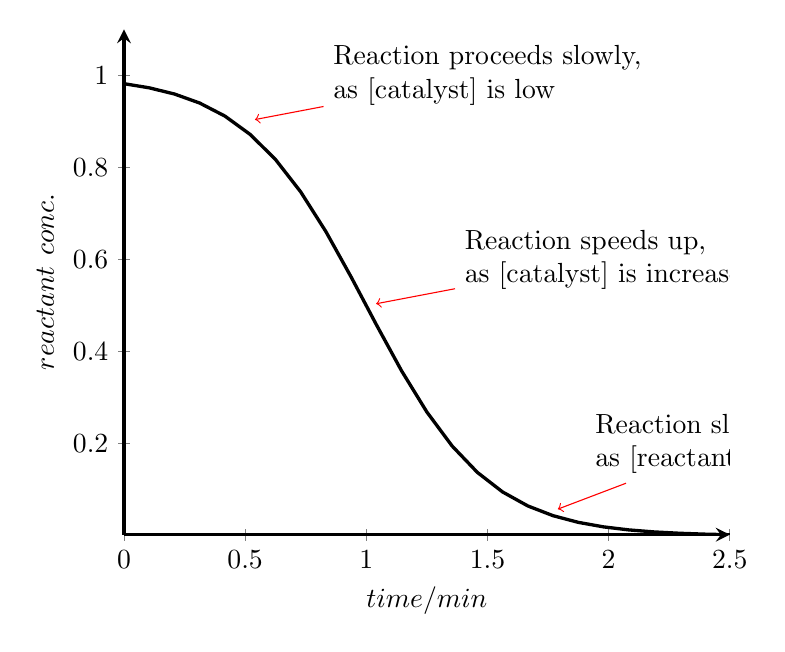
\begin{tikzpicture}

				\begin{axis}[
					axis lines		= left,
					domain			= 0:2.5
					,
					xlabel			= \textbf{$time/min$},
					ylabel			= \textbf{$reactant$ $conc.$},
					axis line style	= very thick,
					height			= 80mm,
					ymax			= 1.1
					% enlarge y limits = 0.15
				]

					\addplot[color = black, very thick]{
						1 - (1 / (1 + e^(-(4*x - 4))))
					};

					\node[align=left] (Sone) at (axis cs:1.5,1){Reaction proceeds slowly,\\as [catalyst] is low};
					\node[align=left] (Stwo) at (axis cs:2.0,0.6){Reaction speeds up,\\as [catalyst] is increases};
					\node[align=left] (Sthree) at (axis cs:2.5,0.2){Reaction slows down,\\as [reactant] decreases};

					\node (Done) at (axis cs:0.5,0.9){};
					\node (Dtwo) at (axis cs:1,0.5){};
					\node (Dthree) at (axis cs:1.75,0.05){};


					\draw[->, red](Sone) -- (Done);
					\draw[->, red](Stwo) -- (Dtwo);
					\draw[->, red](Sthree) -- (Dthree);



				\end{axis}

			\end{tikzpicture}
			\end{center}

			Initially, the rate of reaction is limited by the concentration of the catalyst. As the reaction progresses, more catalyst
			is produced, increasing the rate. Finally, when the reactants are mostly consumed, they become the limiting reactant, and the
			rate of reaction slows once more.

		% end subsection



		\subsection{Biological Catalysis}
			Enzymes are biological catalysts that play an important role in the perpetuation of life. Given that the temperature of the
			reaction system is usually at or near room temperature (~\SI{35}{\celsius} for humans), and that the concentration of reactants
			is usually very low, efficient catalysts are required for reactions to take place at any appreciable rate.

			There are a multitude of different enzymes that perform a very specific job, because the shape of the enzyme is perfectly suited
			to catalyse only a very small group of molecules.

			Because they are soluble in water, globular enzymes typically operate in the same phase as the reactants they catalyse. However, the
			mechanism of action is typical of a heterogeneous reaction, with a limited number of active sites. Thus, they have the characteristics
			of both homogeneous and heterogeneous catalysts.

			\imgdiagram{140mm}{../figures/physical/ch04/enzyme_catalysis.png}{\vspace{-2em}}

			The reactant that is being adsorbed is known as the \textit{substrate}, and the diagram above shows the rough mechanism of the
			enzyme. The fast step of the reaction is almost always the adsorption of the substrate, while the slow, rate-determining step is
			typically the actual reaction of the complex to form the products.


			\subsubsection{Limitations of Enzymes}

				Due to their highly specific and biological nature, enzymes are only efficient at a certain \pH and temperature. In fact,
				going into the extremes of these ranges will irreversibly destroy the enzyme, in a process known as denaturation.

				Furthermore, enzymes, and in fact any heterogeneous catalyst, are prone to poisons --- molecules that are preferentially
				adsorbed onto the active site (either reversibly or irreversibly). These poisons can either slow down the rate of reaction
				significantly if used in high concentrations, or destroy the catalyst all together.

			% end subsubsection

		% end subsection


	% end section
% end part













